\subsection{Fake background measurement}\label{sec:fakes}

The fake lepton background can be predicted by measuring the fake rate for electrons and muons and counting the number of events in the signal region with only candidate id criteria on one of the leptons.

The fake rate is determined as tight-to-loose ratio for leptons on a QCD dominated data sample (selection: $\HT - {\pT}_{lepton} > 200~\GeV, \MET < 20~\GeV, n_{leptons} = 1$). The loose lepton candidate selection is obtained by demanding all usual lepton id criteria except isolation. Figures \ref{fig:fakerateElectrons} and \ref{fig:fakerateMuons} show the fake rate in dependence of the lepton \pT.


\begin{figure}[hbtp]
  \subfigure[]{\label{fig:fakerateElectrons}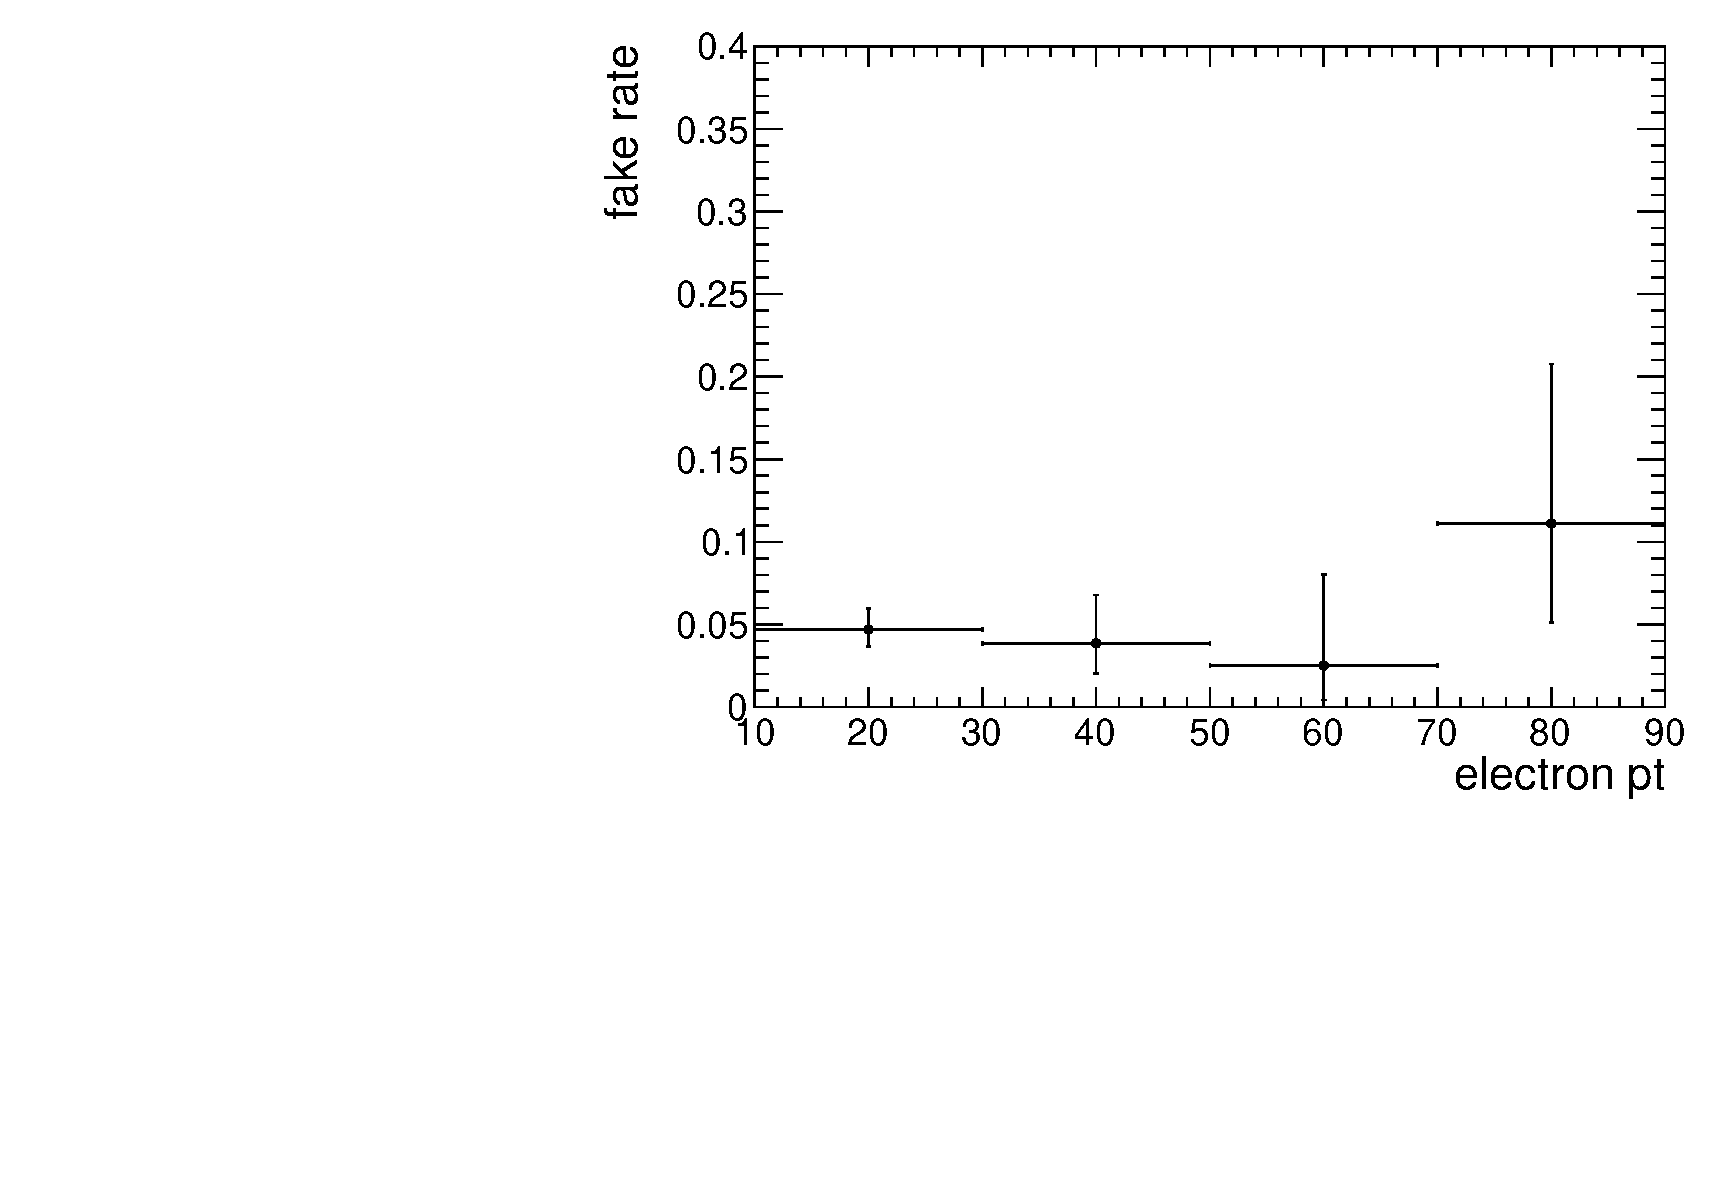
\includegraphics[width=0.49\textwidth]{fakerateElectron.pdf}}\hfill
  \subfigure[]{\label{fig:fakerateMuons}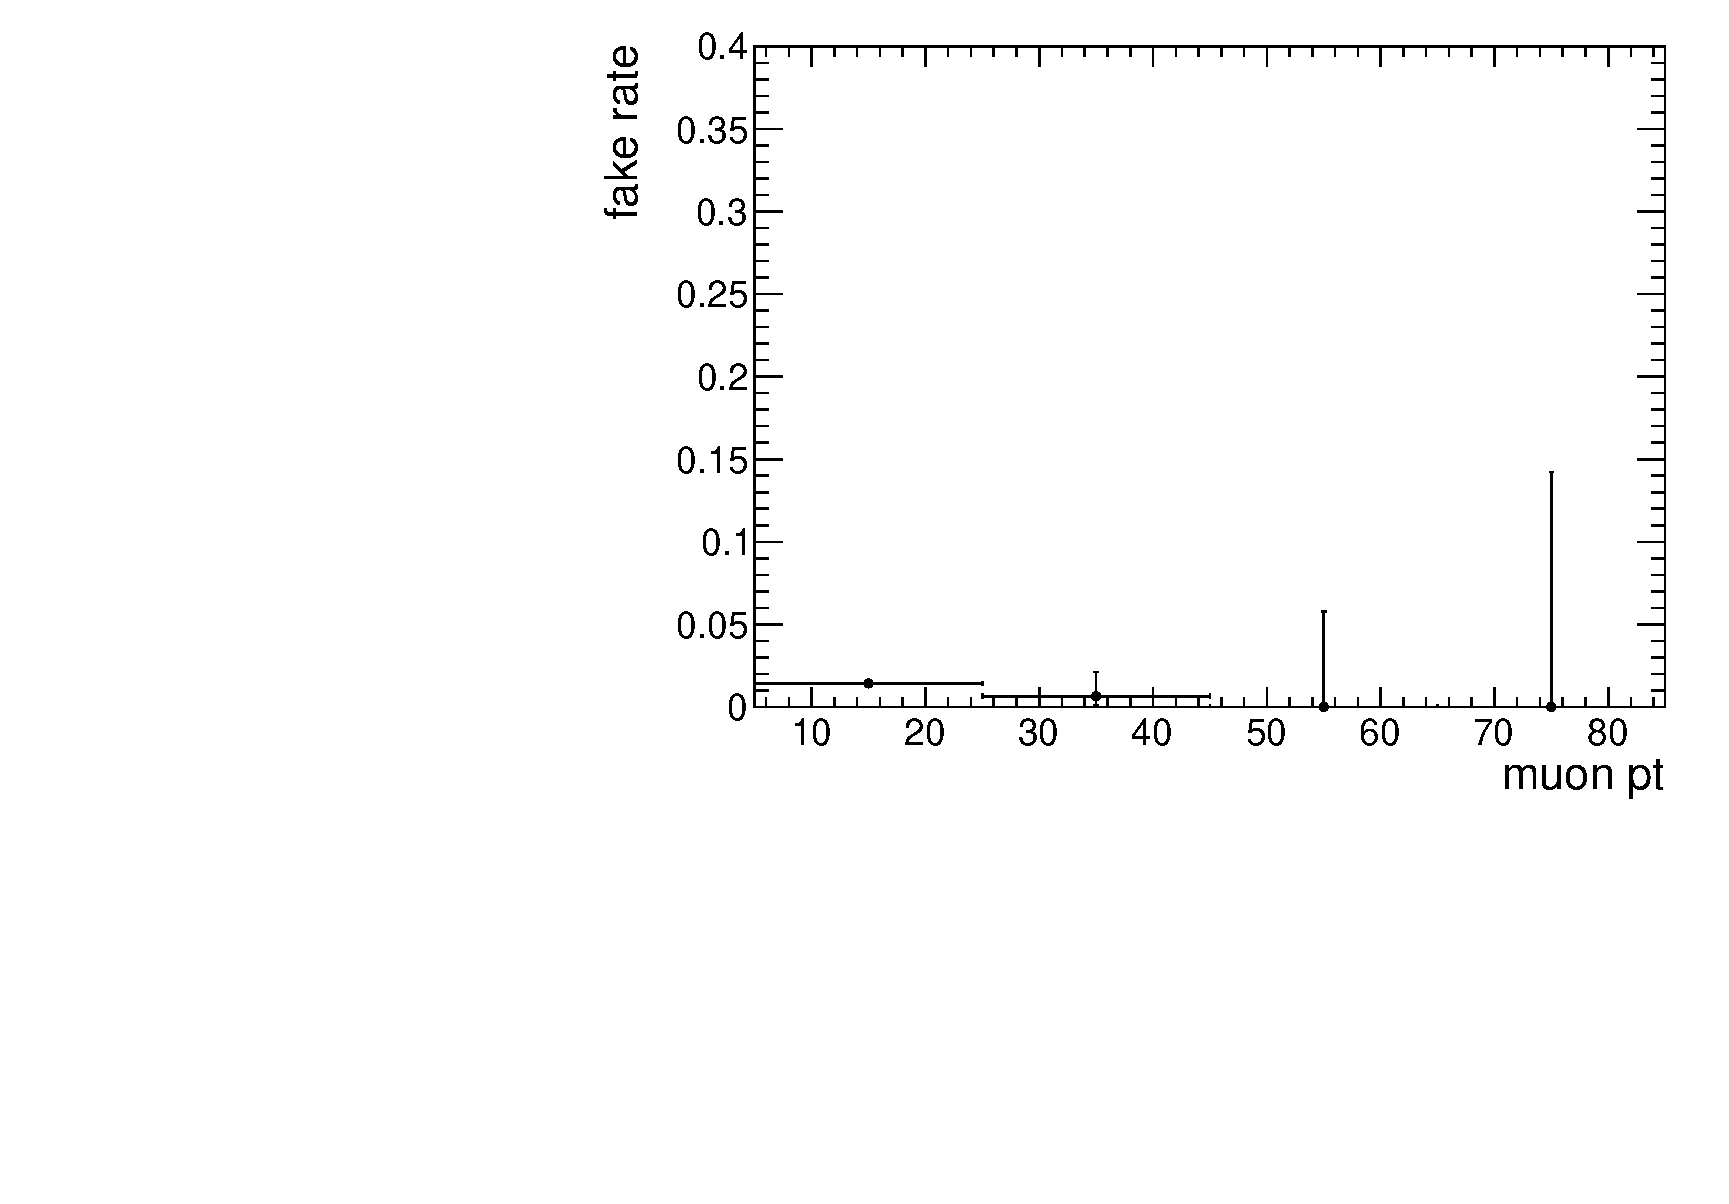
\includegraphics[width=0.49\textwidth]{fakerateMuon.pdf}}\hfill
  \caption{Fake rates for electrons \subref{fig:fakerateElectrons} and muons \subref{fig:fakerateMuons}.}
\end{figure}

To determine the number of expected events that are caused by fake leptons in the signal region, the id criteria cut for one lepton is loosened to select all lepton candidates (no isolation cut). The obtained signal yields are multiplied with the probability that the lepton candidate is not a prompt lepton, but passes the tight lepton selection, $P_{fake}$:

$$P_{fake} = \frac{FR}{1- FR}$$

Table \ref{tab:fakeYields} shows the number of expected background events in the previously defined signal and control regions that are determined using this method.

\begin{table}[hbtp]
\caption{Expected background events due to fake leptons.}
\label{tab:fakeYields}
\begin{center}
\begin{tabular}{c||c|c|c} \hline
Region   & $ee$ & $e\mu$ &  $\mu\mu$  \\
lepton $\pT > (20, 10)~\GeV$  & & & \\\hline \hline
$\HT > 100~\GeV, \MET > 100~\GeV$ &  0.68  & 9.26 & 1.01 \\
$\HT > 350~\GeV, \MET > 150~\GeV$ &  0.14  & 0.52 & 0.07 \\
$\HT > 600~\GeV, \MET > 100~\GeV$ &  0.05  & 0.25 & 0.01 \\
$\HT > 250~\GeV, \MET > 250~\GeV$ &  0.00  & 0.31 & 0.01 \\\hline
\end{tabular}
\end{center}
\end{table}
